
\section*{Exercise 5}
\label{sec:exercise5}

\subsection*{(a)}
\label{sec:a-4}

The dot diagrams\footnote{Jag är lite osäker på hur dot diagram ska se
  ut. Och framföralt hur man gjorde ett i \texttt{matlab}, men jag
  hoppas att detta illusterar det du är ute efter.} are shown in Figure \ref{fig:ex5-marginalplots}. 

\begin{figure}[h]
  \centering
  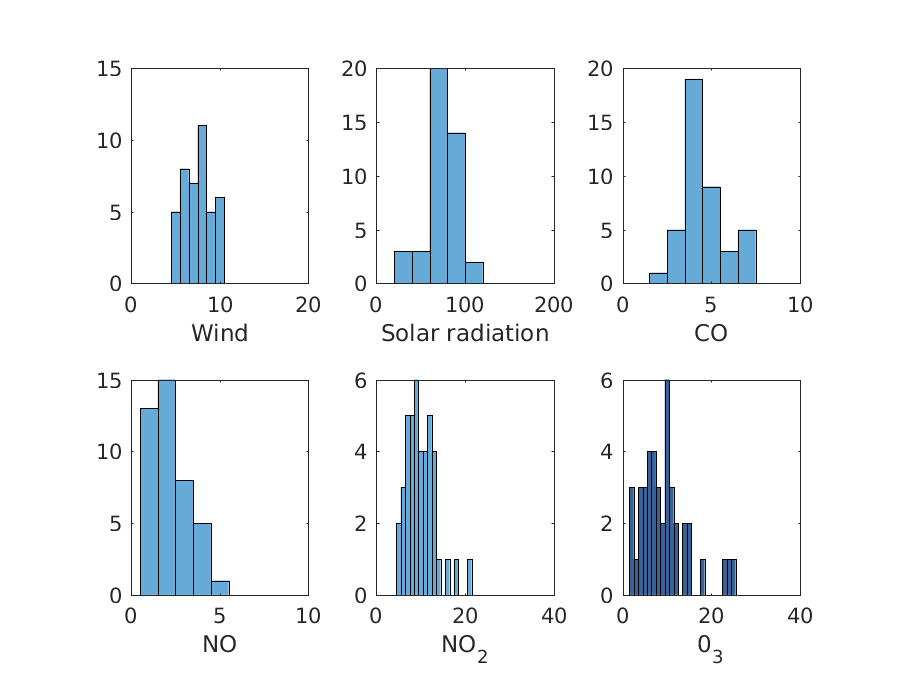
\includegraphics[width=13cm]{ex5-marginalplots}
  \caption{The marginal dot diagrams for all variables}
  \label{fig:ex5-marginalplots}
\end{figure}

\subsection*{(b)}
\label{sec:b-4}

The sample mean is given as
\begin{equation*}
  \bar{x} =
  \begin{pmatrix}
    7.50 & 73.86 & 4.55 & 2.19 & 10.05 & 9.40 & 3.10 
  \end{pmatrix}^T
\end{equation*}
and the sample covariance matrix is
\begin{equation*}
  \b S =
  \begin{pmatrix}
    2.50 & -2.78 & -0.38 & -0.46 & -0.59 & -2.23 & 0.17 \\ 
    -2.78 & 300.52 & 3.91 & -1.39 & 6.76 & 30.79 & 0.62 \\ 
    -0.38 & 3.91 & 1.52 & 0.67 & 2.31 & 2.82 & 0.14 \\ 
    -0.46 & -1.39 & 0.67 & 1.18 & 1.09 & -0.81 & 0.18 \\ 
    -0.59 & 6.76 & 2.31 & 1.09 & 11.36 & 3.13 & 1.04 \\ 
    -2.23 & 30.79 & 2.82 & -0.81 & 3.13 & 30.98 & 0.59 \\ 
    0.17 & 0.62 & 0.14 & 0.18 & 1.04 & 0.59 & 0.48 \\ 
  \end{pmatrix}
\end{equation*}

\subsection*{(c)}
\label{sec:c-4}

The model used was
\begin{equation*}
  y_1 = \beta_0 + \beta_1 x_1 + \beta_2 x_2 + \epsilon,
\end{equation*}
where $\hat{\beta} = (10.1145,\   -0.2113,\    0.0205)$, then the
residual sum of squares is
\begin{equation*}
  \b \epsilon^{T} \b \epsilon = 455.1356.
\end{equation*}
This is give the $R^{2} = (\b \hat \beta^{T} \b x)^{T} (\b \hat
\beta^{T} \b x)/(\b Y^{T} \b Y) = 0.9033$, which is close to 1, and so
we get an indication that the model fits the data well. 
Further, a prediction interval can be constructed using
\begin{equation*}
  \mean y \pm \sqrt{s^{2}}t_{df}(1 - \alpha/2)\sqrt{1 + \b q (\b x^{T} \b
    x)^{-1}\b q^{T}},
\end{equation*}
where $\mean y = \b \hat \beta^{T} \b q$, $s^{2} =\b \epsilon^{T} \b \epsilon / (df - 2) $, $df = n - k - 1
= 40$ is the degrees of freedom, and $\b q = (1, 10, 80)^{T}$ represents
the point $(z_{1}, z_{2}) = (10, 80)$.  We get the prediction interval
(with $\alpha = 0.05$)
\begin{equation*}
  \begin{pmatrix}
    2.52 &16.77 
  \end{pmatrix}.
\end{equation*}

\subsection*{(d)}

Here, we propose the linear model
\begin{equation*}
  \begin{pmatrix}
    \b y_1 & \b y_2
  \end{pmatrix} = 
  \b X\b B + \b E,
\end{equation*}
where 
\begin{equation*}
 \b X =
  \begin{pmatrix}
    \b 1_n & \b x_1 & \b x_2
  \end{pmatrix}.
\end{equation*}
We found that
\begin{equation*}
 \b \hat  B =
  \begin{pmatrix}
    10.11 & -0.21 \\ 
    0.02 & 8.28 \\ 
    -0.79 & 0.10 
  \end{pmatrix}.
\end{equation*}
With the sum or squared errors being
\begin{equation*}
  \b E ^{T} \b E = 
  \begin{pmatrix}
    455.14 &82.91 \\ 
    82.91 &1077.97
  \end{pmatrix},
\end{equation*}

and
\begin{equation*}
  \b \Sigma = \frac{1}{n-r-1} \b E ^{T} \b E = 
  \begin{pmatrix}
    11.38 &2.07 \\ 
    2.07 &26.95  
  \end{pmatrix},\quad \rank X = r+1
\end{equation*}
and the $R^{2}_{ij}$ values, where $R^{2}_{ij} =  \hat Y_{i}^{T} 
\hat Y_{j} /  Y_{i}^{T} Y_{j}$, we get
\begin{equation*}
  \b R^{2} =
  \begin{pmatrix}
    0.90 &0.98 \\ 
    0.98 &0.78
  \end{pmatrix},
\end{equation*}
where all elements are fairly close to 1, which gives and indication
that the model fits well. We can construct a prediction interval for
$x_{1} = 10$, and $z_{2} = 80$ if we find the vectors $\b y =
(y_{1}, y_{2})^{T}$ that
satisfies
\begin{align*}
  \left(
    \frac{\b \hat B^{T} \b q - \b y}{\sqrt{1 + \b q^{T}(\b X^{T} \b
        X)^{-1}\b q}}
  \right)^{T} &
  \left(
    \frac{n}{n-r-1}\b \Sigma
  \right)^{-1}
   \left(
    \frac{\b \hat B^{T} \b q - \b y}{\sqrt{1 + \b q^{T}(\b X^{T} \b
        X)^{-1}\b q}}
  \right)
\leq \\
  &
    \left(
    \frac{m(n-r-1)}{n-r-m}
    \right)
    F_{m,n-r-m}(1-\alpha),
\end{align*}
where $q = (1, 10, 80)^{T}$, and $m$ is the number of responses. The
resulting ellipse is displayed in Figure \ref{fig:ex5-ellipse}. In the
prediction ellipse, the midpoints for $y_{1}$
is the same as in the prediction interval from the exercise above. Also
note that we get a much wider interval in the
prediction interval compared to the prediction region. 

\begin{figure}
  \centering
  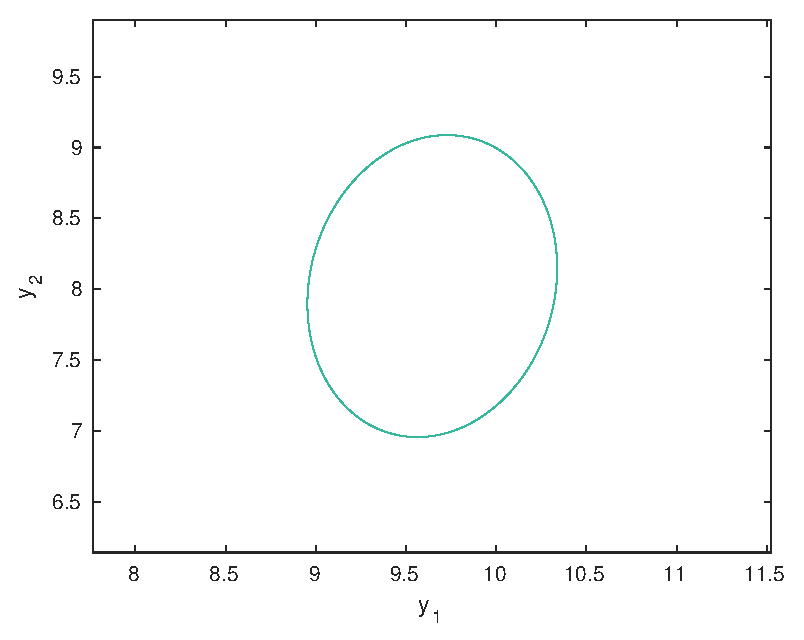
\includegraphics[width=10cm]{ex5-ellipse}
  \caption{The prediction region for $z_1 = 10$, and $z_2 = 80$.}
  \label{fig:ex5-ellipse}
\end{figure}

%%% Local Variables:
%%% mode: latex
%%% TeX-master: "examination"
%%% End:
